% Adapted from the MLSP 2026 poster (column 1): Pavia University patch,
% one background pixel and its spectrum, the target spectrum, and a
% weak target pixel w + 0.15 s.  Coordinates are the poster's, scaled
% through the x/y units so that text keeps the document font size.
\begin{figure}[htbp]
\centering
\begin{tikzpicture}[x=0.5cm, y=0.5cm, line cap=round, font=\footnotesize\linespread{1}\selectfont]
  % ---- Pavia patch (image 13cm on the poster -> 5.46cm here)
  \node[anchor=south west, inner sep=0] at (7.15,0) {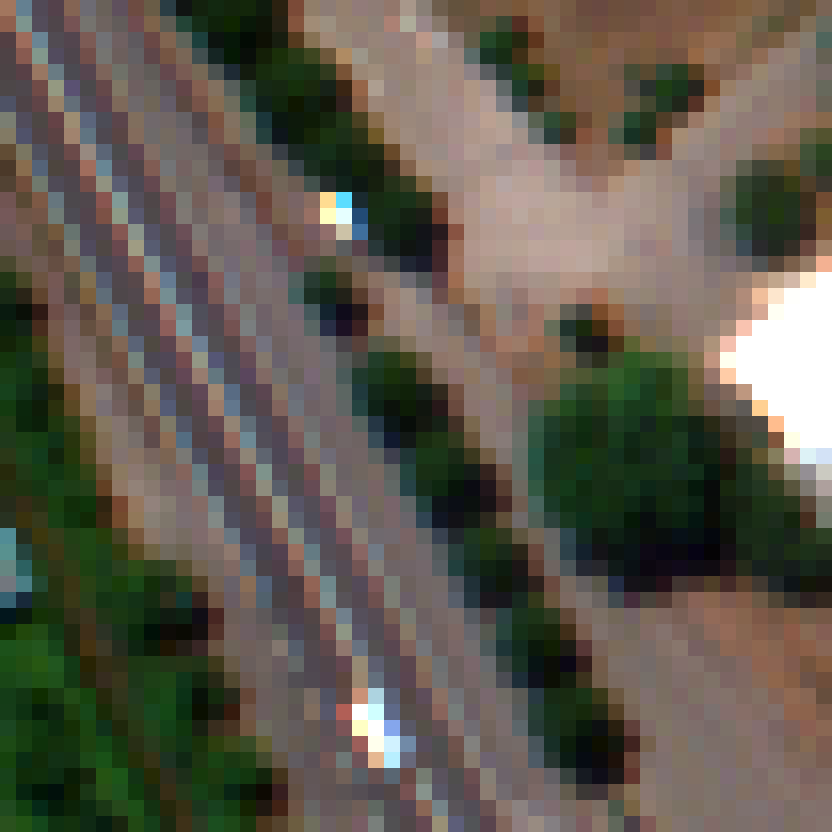
\includegraphics[width=6.5cm]{figures/pavia_patch.png}};
  \draw[pmuted!70, thin] (7.15,0) rectangle (20.15,13);
  % marked background pixel + halo
  \draw[pyellow, line width=1.0pt] (12.90,7.00) rectangle (13.15,7.25);
  \draw[pyellow, line width=0.6pt, dashed] (12.40,6.50) rectangle (13.65,7.75);
  % zoom lines down to the spectrum panel
  \draw[white, line width=2.3pt] (12.40,6.50) -- (1.40,-2.20);
  \draw[white, line width=2.3pt] (13.65,6.50) -- (25.90,-2.20);
  \draw[pyellow, line width=1.3pt] (12.40,6.50) -- (1.40,-2.20);
  \draw[pyellow, line width=1.3pt] (13.65,6.50) -- (25.90,-2.20);
  % ---- spectrum panel (below the image)
  \begin{scope}[shift={(1.4,-8.2)}]
    \draw[pmuted!60, line width=0.6pt] (0,0) -- (24.5,0);
    \draw[pmuted!60, line width=0.6pt] (0,0) -- (0,6.0);
    \draw[pnavy, line width=0.9pt] plot coordinates
      {(0.00,1.35) (0.47,0.79) (0.96,0.69) (1.43,0.71) (1.93,0.66) (2.40,0.59) (2.89,0.60) (3.36,0.54) (3.83,0.54) (4.33,0.56) (4.80,0.60) (5.29,0.66) (5.76,0.72) (6.26,0.80) (6.72,0.85) (7.19,0.88) (7.69,0.88) (8.16,0.81) (8.65,0.78) (9.12,0.70) (9.62,0.71) (10.09,0.68) (10.56,0.66) (11.05,0.65) (11.52,0.62) (12.02,0.61) (12.48,0.60) (12.98,0.58) (13.45,0.54) (13.94,0.54) (14.41,0.54) (14.88,0.54) (15.38,0.56) (15.85,0.70) (16.34,1.01) (16.81,1.50) (17.31,2.01) (17.78,2.69) (18.24,3.33) (18.74,3.76) (19.21,4.10) (19.70,4.14) (20.17,4.06) (20.67,4.21) (21.14,4.19) (21.61,4.12) (22.10,4.10) (22.57,4.10) (23.07,3.94) (23.54,3.96) (24.03,3.81) (24.50,3.94)};
    \draw[pbrown, line width=0.9pt] plot coordinates
      {(0.00,3.17) (0.47,3.39) (0.96,3.89) (1.43,4.21) (1.93,4.44) (2.40,4.71) (2.89,4.86) (3.36,4.99) (3.83,5.05) (4.33,5.05) (4.80,5.02) (5.29,4.96) (5.76,4.92) (6.26,4.88) (6.72,4.71) (7.19,4.60) (7.69,4.42) (8.16,4.25) (8.65,4.05) (9.12,3.80) (9.62,3.50) (10.09,3.19) (10.56,2.97) (11.05,2.81) (11.52,2.69) (12.02,2.60) (12.48,2.56) (12.98,2.50) (13.45,2.46) (13.94,2.48) (14.41,2.51) (14.88,2.59) (15.38,2.62) (15.85,2.68) (16.34,2.73) (16.81,2.73) (17.31,2.66) (17.78,2.59) (18.24,2.61) (18.74,2.66) (19.21,2.75) (19.70,2.78) (20.17,2.76) (20.67,2.80) (21.14,2.78) (21.61,2.80) (22.10,2.82) (22.57,2.90) (23.07,2.95) (23.54,3.01) (24.03,3.06) (24.50,3.15)};
    % target-pixel example: w + 0.15 s (dashed)
    \draw[pteal, line width=0.9pt, dashed] plot coordinates
      {(0.00,1.80) (0.47,1.27) (0.96,1.25) (1.43,1.31) (1.93,1.30) (2.40,1.27) (2.89,1.30) (3.36,1.26) (3.83,1.27) (4.33,1.29) (4.80,1.32) (5.29,1.38) (5.76,1.43) (6.26,1.50) (6.72,1.53) (7.19,1.54) (7.69,1.51) (8.16,1.42) (8.65,1.36) (9.12,1.24) (9.62,1.21) (10.09,1.13) (10.56,1.08) (11.05,1.04) (11.52,1.00) (12.02,0.97) (12.48,0.96) (12.98,0.93) (13.45,0.88) (13.94,0.88) (14.41,0.89) (14.88,0.90) (15.38,0.92) (15.85,1.07) (16.34,1.39) (16.81,1.88) (17.31,2.38) (17.78,3.05) (18.24,3.69) (18.74,4.13) (19.21,4.48) (19.70,4.53) (20.17,4.45) (20.67,4.60) (21.14,4.58) (21.61,4.51) (22.10,4.49) (22.57,4.51) (23.07,4.35) (23.54,4.38) (24.03,4.24) (24.50,4.38)};
    \node[fill=white, inner sep=1pt, text=pnavy, anchor=west] at (17.6,0.58) {background $w$};
    \node[text=pteal, anchor=south east] at (24.3,4.72) {target pixel $= w + 0.15\, s$};
    \node[text=pbrown, anchor=south west] at (6.0,5.35) {$s$ -- known target spectrum};
    \node[text=pbody, anchor=north] at (12.25,-0.30) {spectral band $1,\ldots,d$};
  \end{scope}
\end{tikzpicture}
\caption{The additive model on real data. Top: a pseudo-color patch of the
Pavia University scene, where each pixel is a $103$-dimensional spectral
vector. Bottom: the spectrum $w$ of the marked background pixel, the known
target spectrum $s$, and the resulting weak target pixel $w+0.15\,s$.}
\label{fig:pavia_patch}
\end{figure}
